% !TEX root = trackjet_intnote.tex

This section gives an overview of the sources of systematic uncertainties on the \pp\ and \pbpb\ charged particle spectra associated with jet. The sources of systematic uncertainties in the measurement are the following and are further described below:

\begin{itemize}

\item Jet energy scale

\item Jet energy resolution

\item Track selection

\item Truth track definition

\item Detector material description in simulation

\item Tracking in dense environments

\item Fake track subtraction

\item Track momentum

\item Unfolding

\item Underlying event contribution

%\item MC non-closure

\end{itemize}


The systematic uncertainties on the \Rdptr\ distributions for a selection of track \pt\ ranges (1.0--1.6 \GeV, 2.5--4.0 \GeV, 6.3--10 \GeV) in jets with \pt\ in the 126--158 \GeV\ range are shown in Figure~\ref{fig:rdptr_sys_uncert}. All uncertainties are assumed to be uncorrelated, and thus are combined in quadrature to give the total systematic uncertainty. The systematic uncertainties for other jet \pT\ interval as show in appendix\ref{sec:appendixA}. 

\begin{figure}
\centering{
\begin{tabular}{cc}
	 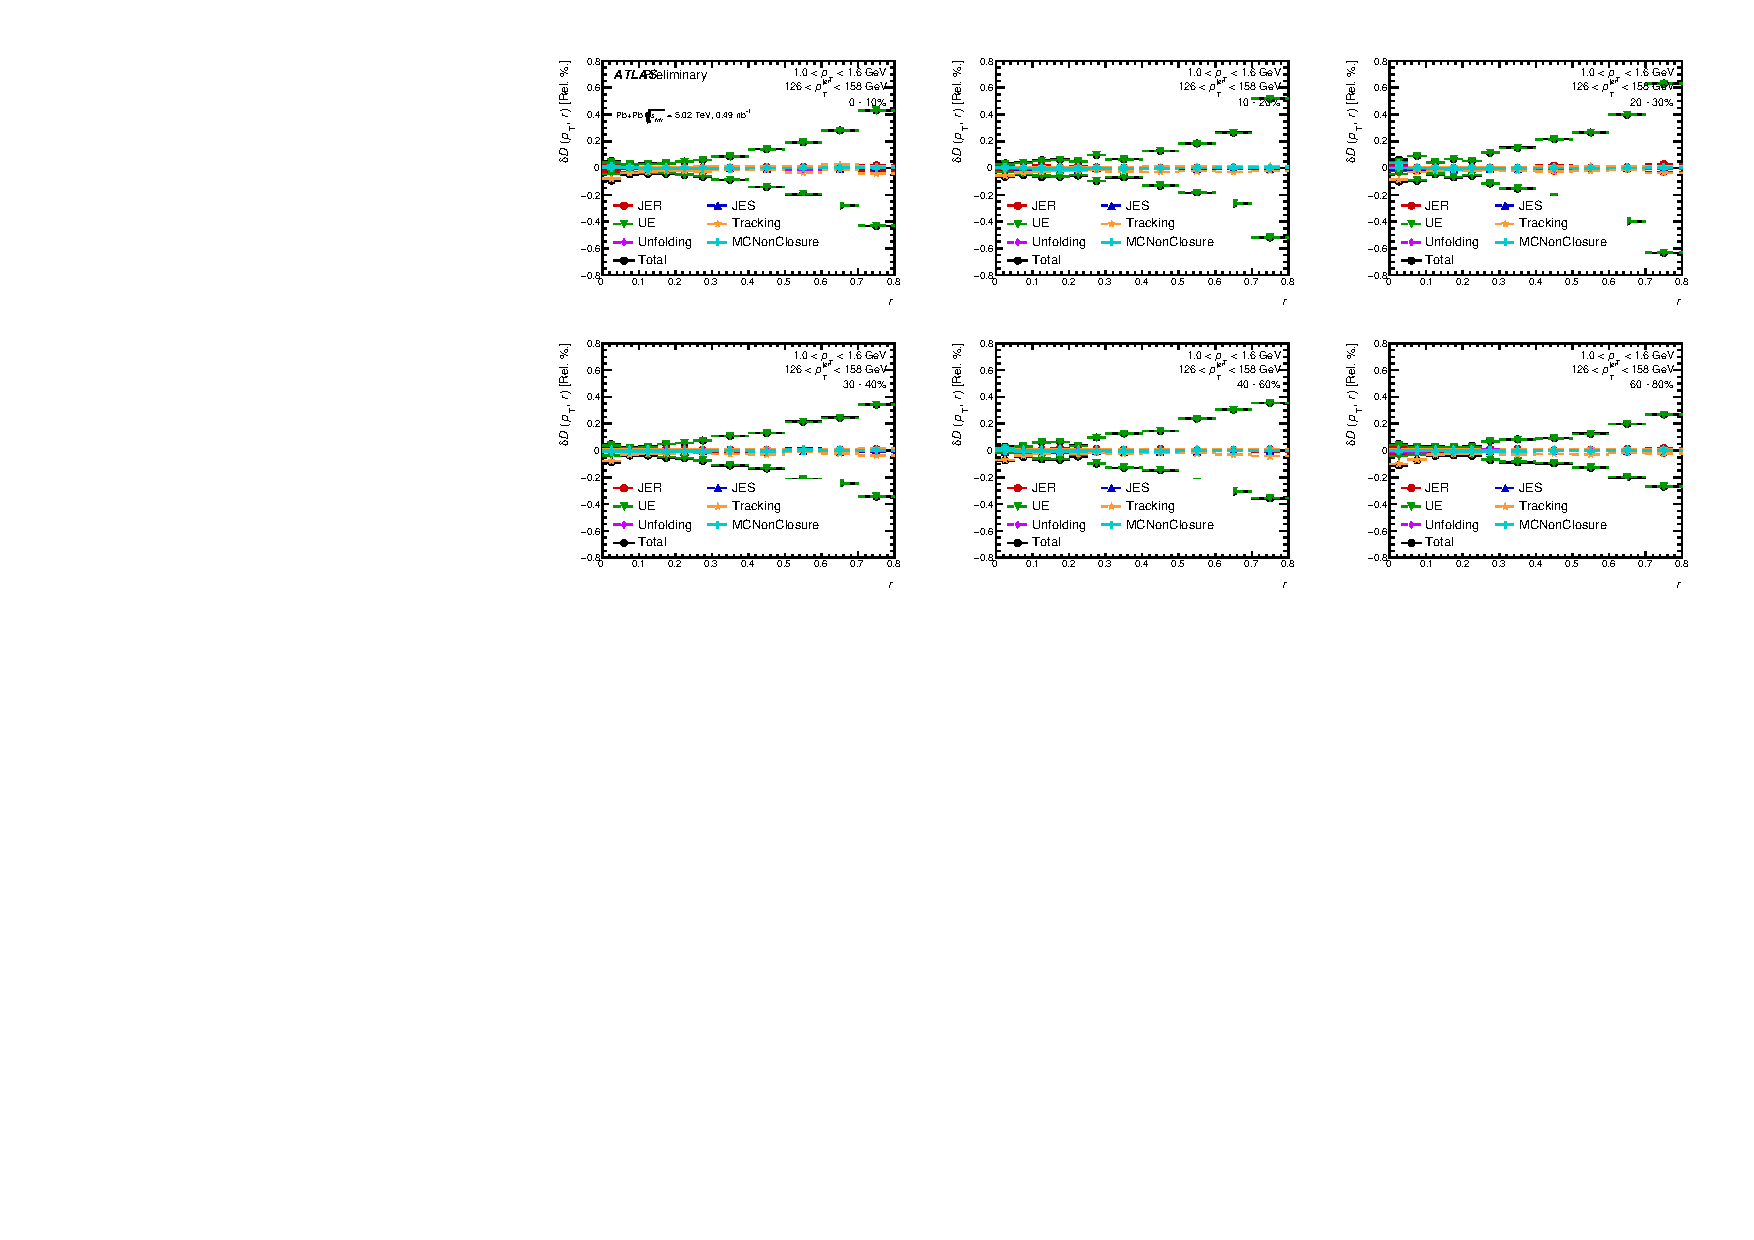
\includegraphics[page=1, width=0.50\textwidth]{figures_systematics/ChPS_dR_sys_PbPb_error} 	
	 \includegraphics[page=3, width=0.50\textwidth]{figures_systematics/ChPS_dR_sys_PbPb_error} \\
	 \includegraphics[page=5, width=0.50\textwidth]{figures_systematics/ChPS_dR_sys_PbPb_error} 
	 \includegraphics[page=6, width=0.50\textwidth]{figures_systematics/ChPS_dR_sys_PbPb_error} \\
\end{tabular} }
   \caption{A summary of the systematic uncertainties on \RDptr\ distributions for different track \pt, bins, for jets with \pt\ 125--158 \GeV\ , as a function of \rvar\ for different centrality bins. The uncertainties from the JES, JER, UE, and Tracking  are shown, along with the total systematic uncertainty from all sources. }
      \label{fig:rdptr_sys_uncert}
\end{figure}




The systematic uncertainties have been evaluated separately for \Dptr\ distributions and for their ratios, as a function of jet \pT\ for \pp\ and \pbpb\ collisions. For each systematic variation, the entire unfolding procedure is repeated (2D unfolding of the fragmentation
functions as a function of \ptjet\, the 1D unfolding of the single \ptjet\ spectrum and the bin-by-bin correction for position resolution). This is necessary because the jets are in both the 2D and the 1D unfolding procedures and must be treated in a consistent manner throughout the analysis (e.g. a shift in the JES should 
shift jets in the fragmentation functions as a function of \ptjet\ in the same manner
that the single jet spectrum itself is shifted).
The positive relative uncertainty was used to calculate the upper bound of the systematic uncertainty, whereas the negative relative uncertainty was used to calculate the lower bound. All sources of systematic uncertainty discussed in this section are treated as mutually uncorrelated and are combined in quadrature to obtain the total systematic uncertainty. 

\subsection{Jet energy scale uncertainty}

The uncertainty on the JES for heavy ion jets has two parts.  The first is taken from
 \pp\ JES uncertainties for EMTopo jets while the second is specific to the heavy ion jets
and collision energies (for flavor related uncertainties).  For the \pp\ part we use the strongly reduced
set of 4 nuisance parameters (in Scenario 1) as described in Ref.~\cite{JESuncertaintytwiki}. Nuisance parameters that are not applicable for HI jet collections (pileup, b-jets, flavor and MC non closure) are removed or replaced (flavor uncertainties). The heavy ion specific components are from the cross calibration~\cite{cc2015} and the jet
flavor uncertainties at 5.02~TeV~\cite{pPbIntNote}.  For each component of the variation
the response matrices are regenerated with the shifted \ptjet:
\begin{equation}
   \pT^{\star,\mathrm{reco}} = \pT^{\mathrm{reco}} (1\pm U^{\mathrm{JES}}(\pT , \eta)).
\end{equation}
The data is then re-unfolded with these response matrices and the variation in the fragmentation 
functions is taken as the systematic uncertainty.

 The centrality dependent uncertainty on the JES was evaluated by shifting the jet \pt\ of all measured jets up and down by shift between 0\% and 0.5\%. The magnitude of the shift depends on the centrality in the way that the uncertainty on the jet \pt\ is 0.5\% in 1\% most central collisions and than linearly decreases to 0\% in 60\% peripheral bin. The size of the shift reflects the uncertainty on the JES evaluated as using the $r-$track study where the sum of \pT\ of the tracks associated to a reconstructed jet is compared to the reconstructed jet \pT\ in ratio that is than compared between PbPb data and MC~\cite{HIjesnote,PbPbRaaNote}.

\subsection{Jet energy resolution}
To account for systematic uncertainties due to disagreement between the jet energy resolution in data and MC, the unfolding procedure was repeated with a modified response matrix. The matrix was generated by repeating the MC study with modifications to the $\Delta \pt$ for each matched truth-reconstructed jet pair. 



     The procedure to generate modified migration matrices follows the standard procedure applied in p+p jet measurements 
     and is used for both the \pp\ and \pbpb\ collisions. 
     The $\texttt{JetEnergyResolutionProvider}$ tool~\cite{JERUncertaintyProviderRun2} was used to 
     retrieve uncertainty on the fractional resolution, $\sigma^{\mathrm{syst}}_{\mathrm{JER}}$ as a function of jet $\pt$ and $\eta$. An additional HI jet specific uncertainty from the cross calibration of the HI jet collections ~\cite{cc2015} is applied to jets in both \pp\ and \pbpb\ collisions.
     The full JER uncertainty on 2015 \pp\ data is shown also in Ref.~\cite{Aad:1696485}

     The jet $\pt^{\mathrm{reco}}$ was then smeared by
     \begin{equation}
	\pt^{\star, \mathrm{reco}} = \pt^{\mathrm{reco}}\times \mathcal{N}(1,\sigma^{\mathrm{eff}}_{\mathrm{JER}})\,,
     \end{equation}
     where $\mathcal{N}(1,\sigma^{\mathrm{eff}}_{\mathrm{JER}})$ is the normal distribution with the effective resolution $\sigma^{\mathrm{eff}}_{\mathrm{JER}}=\sqrt{(\sigma_{\mathrm{JER}} + \sigma^{\mathrm{syst}}_{\mathrm{JER}})^{2} - \sigma_{\mathrm{JER}}^{2}}$.
%      As this smearing is random the procedure is repeated 10 times.

     %The systematic uncertainties on the \Dptr\ distributions decreases with decreasing \pt\ and increasing jet \pT. The typical systematic uncertainty originating from JER changes varies from 10\% to 1\% depending on the jet \ET\ and $z$. 


\subsection{Track selection and efficiency}

\paragraph{Track selection}  This uncertainty was estimated by tightening the tracking cuts by adding the cuts
on the significance of $d_0$ and $z_0$ as described in the Section~\ref{sec:trackselection}.  
The entire analysis is redone with these track selections (including re-deriving the tracking efficiencies and the $\eta-\phi$ maps for the UE estimation) and the difference from the nominal analysis is taken as the systematic uncertainty. 


%\paragraph{Tracking efficiency fits}  This uncertainty comes from the statistical uncertainty on the fits
%used to parameterize the efficiency corrections.  Since this uncertainty is largely from the statistical 
%fluctuations of the uncertainty points it is taken to be uncorrelated between \pp\ and \pbpb. 
%This uncertainty is not yet added to the total systematics for fragmentation functions in \pbpb\ collisions.

\paragraph{Truth track definition}  
This uncertainty quantifies robustness of the matching of reconstructed to truth particles.
The uncertainty is taken as a difference in the final results obtained with  $MCprob>$ 0.3 
and results obtained with $MCprob>$ 0.5. This systematic included a re-derivation of the $\eta-\phi$ maps for UE estimation. The change in tracking efficiency is negligible.


\paragraph{Detector material description in simulation}
The uncertainty on the inner detector material
varies with \pttrk\ and \etatrk\ from 0.5\% to 2.0\%~\cite{ref:tracktwiki} on the efficiency correction. This systematic also included a re-derivation of the $\eta-\phi$ maps for UE estimation.


\paragraph{Tracking in dense environments}
There is a 0.4\% uncertainty on the efficiency due to tracking in dense environments (the core of the jet)~\cite{ref:tracktwiki}. This systematic also included a re-derivation of the $\eta-\phi$ maps for UE estimation.


\paragraph{Fake rate}
The uncertainty on the rate of fake tracks is 30\% independent of \pttrk\ and \etatrk~\cite{ref:tracktwiki}. 

\paragraph{Uncertainty on the track momentum}
To account for a possible miss-alignment in \pp\ and \PbPb\ data, the reconstructed \pT\ of each track (corrected first as described in section~\ref{Sec:Trackmomentumcorrection}) was changed according to~\cite{TrackingRec}:

\begin{equation}
\pt \rightarrow \pt \times (1 + q \times \pt \delta_{sagitta}(\eta, \phi))^{-1},
\end{equation}
where $q$ is charge of the track and $\delta_{sagitta}(\eta, \phi)$ is uncertainty on the track curvature. The uncertainty derived for 5.02~TeV \pp\ and \PbPb\ data is included in InDetTrackSystematicsTools-00-00-19. Due to statistical origin of the uncertainty the resulting systematic uncertainty is symmetrized. This systematic also included a re-derivation of the $\eta-\phi$ maps for UE estimation.

%The resulting systematic uncertainty is $<<1$\% for low and intermediate $z$ and \pT\ and reaches up to 4\% at high $z$. As the source of the shift is present both in \pp\ and \PbPb\ it does partially cancel in the ratios.  

\subsection{Systematic uncertainty due to unfolding}
The systematic uncertainty associated with the unfolding is connected with the sensitivity of the unfolding procedure to the choice of the input distributions. The systematic is evaluated by generating response matrices from the MC distributions without the reweighting factor that is used to match the jet spectrum and \Dptr\ distributions in data, and then unfolding the data using these response matrices. This has minimal effect on track \pt\ because of the good track momentum resolution in the kinematic region of interest. The uncertainty is evaluated by comparing the nominal result with the un-reweighed result, and is considered to be uncorrelated between \pbpb\ and \pp.


\subsection{Systematic uncertainty due to the UE event subtraction}
The systematic uncertainty associated with the estimation of the UE has two main components: one is the statistical uncertainty on the $\eta-\phi$ maps used in the map method (described in section~\ref{sec:map_method}) , and the other is the comparison of the map method to the alternative cone method (described in section~\ref{sec:cone_method}. More details on the cone method can be found in Ref.~\cite{PbPb5TeVIntNote}. 

\subparagraph{Uncertainty from map statistic:} 
The $\eta-\phi$ maps used in the estimation of the underlying event are sparsely populated for high track \pt\ and high \ptjet, and are susceptible to statistical fluctuations. To take this into account, 100 pseudo-experiments are conducted to re-estimate the set of maps, with a bin-by-bin gaussian variation where the mean and standard deviation were taken to be the bin content and bin error from the nominal set of maps. The distribution of the relative difference between each estimation of the shifted underlying event and and the nominal value ( $\delta (\mathrm{UE}) = \mathrm{GausWidth}(\mathrm{UE}_i - \mathrm{UE}_{\mathrm{nominal}} / \mathrm{UE}_{\mathrm{nominal}})$ is fit to a gaussian, and the width is taken to be the systematic uncertainty. This uncertainty is symmetrized to be conservative.  A few examples of the distribution of normalized relative differences can be seen in Fig. \ref{fig:gaus_diff}. The size of the systematic from this can be seen in Fig.\ref{fig:mapstat_corr}.

\begin{figure}
\centering{
\begin{tabular}{cc}
	 \includegraphics[width=0.55\textwidth]{figures_systematics/g0} &
	 \includegraphics[width=0.55\textwidth]{figures_systematics/g1} \\
	 \includegraphics[width=0.55\textwidth]{figures_systematics/g2} &
	 \includegraphics[width=0.55\textwidth]{figures_systematics/g3} \\
\end{tabular} }
   \caption{Examples of the relative differences between the nominal and shifted values of the underlying event, fit to a gaussian distribution. The width on the gaussian is taken as the systematic uncertainty on the underlying. Wider distributions indicate a larger statistical uncertainty on the bin content in the $\eta-\phi$ map used to estimate the UE.}
      \label{fig:gaus_diff}
\end{figure}

\begin{figure}[h]
    \centerline{
       \includegraphics[width=0.75\textwidth]{figures_systematics/mapStatCorrection}
    }
    \caption{Size of the systematic uncertainty from the map statistic component, as a function for \rvar\ for 0-10\% \pbpb\ collisions, in 126-158 GeV jets, 1-1.6 GeV tracks.}
    \label{fig:mapstat_corr}
 \end{figure}




\subparagraph{Uncertainty from cone method:} The difference between the two methods is shown in Fig.~\ref{fig:conemethod_corr} and is found vary slowly with \ptjet\ and track \pT. There is a  small centrality dependence, which is coming from fact that the underlying event strongly depends on the centrality.
This uncertainty is conservatively symmetrized. The absolute size of the uncertainty on the UE is typically small however due to small signal-to-background ratio it is the dominant systematic uncertainty in central collisions, for lowest \pT\ tracks, and large \rvar.

\begin{figure}
\centerline{\includegraphics[page=2,width=1.\textwidth]{figures_systematics/UE_x_ratio}}
    \caption{Size of the systematic uncertainty from the cone method, as a function for \rvar\ for 0-10\% \pbpb\ collisions, in 126-158 GeV jets, 1-1.6 GeV tracks.}
    \label{fig:conemethod_corr}

\end{figure}


\subsection{MC non-closure}
To make sure that all the sources of systematic uncertainties were covered the systematic uncertainty from the non-closure�� in the MC was also evaluated. It was 
calculated as a deviation from unity of ratios of fully corrected and reconstructed charged particle distributions in MC to the charged particle distributions
evaluated at the truth level. 
This uncertainty can be considered a measure of unknowns in the analysis, but it also includes fluctuations due to 
the finite statistics in the MC which are used to evaluate it (especially in high \pttrk\ regions of
the analysis. The non-closure can be seen in Fig.~\ref{fig:pbpbclosure}).  
The systematic uncertainty is taken to be uncorrelated between \pbpb\ and \pp 


\begin{figure}
\centerline{\includegraphics[page=2,width=1.\textwidth]{figures_systematics/UE_x_ratio}}
    \caption{Size of the systematic uncertainty from the cone method, as a function for \rvar\ for 0-10\% \pbpb\ collisions, in 126-158 GeV jets, 1-1.6 GeV tracks.}
    \label{fig:pbpbclosure}

\end{figure}
\subsection{Correlations between the systematic uncertainties in \pbpb\ and \pp\ collisions}

Due to the common analysis and reconstruction procedure, and detector conditions, the systematic uncertainties are correlated between the \pp\ and
\pbpb\ collisions in most cases. Table~\ref{tab:systematics} summarizes correlations between \pp\ and \PbPb\ and also point-to-point correlations of individual distributions. The unfolding uncertainty is uncorrelated between the two systems because it
comes from the sensitivity of the unfolding to the starting MC distribution. In \pbpb\ collisions where the fragmentation is modified by the presence of the QGP, this sensitivity could be different than in \pp\ collisions where the fragmentation functions are quite similar to those in \pythiaeight~\cite{Aaboud:2017tke}. The impact of the modification of the fragmentation process in \PbPb\ compared to \pp\ and MC simulations is account for in the HI specific data-driven and centrality dependent uncertainty on the JES.

\begin{table}[h]
\begin{center}
\begin{tabular}{|c|c|c|c|}
\hline
uncertainty & \pp\ and \PbPb\ correlated & point-to-point correlated & one/two sided or symmetrized \\ \hline
JES (\pp) & yes & yes & two sided \\ \hline
JES (HI) & no & yes & two sided \\ \hline
JER & yes & yes & symmetrized \\ \hline
Track selection & yes & yes & one sided \\ \hline
Truth track definition & yes & yes & one sided \\ \hline
Material & yes & yes & one sided \\ \hline
Dense environment & yes & yes & one sided \\ \hline
Fake rate & yes & yes & symmetrized \\ \hline
Track momentum & yes & no & two sided \\ \hline
Unfolding & no & yes & one sided \\ \hline
UE subtraction & no & yes & symmetrized \\ \hline
% MC non-closure & no & no & symmetrized \\ \hline
\end{tabular}
\caption{Summary of correlation of different systematic uncertainties.}
\label{tab:systematics}
\end{center}
\end{table}

In the case where the systematic uncertainties are correlated, we evaluate \Rdptr\ ratios using the systematic variation from the nominal distributions in both \pp\ and \pbpb. The variation in the ratio is used as the systematic uncertainty. The variations in the ratios are summed in quadrature to get the total systematic uncertainty on the ratio.


